%  LaTeX support: latex@mdpi.com 
%  For support, please attach all files needed for compiling as well as the log file, and specify your operating system, LaTeX version, and LaTeX editor.

%=================================================================
\documentclass[sensors,article,submit,pdftex,moreauthors]{Definitions/mdpi} 
%\documentclass[preprints,article,submit,pdftex,moreauthors]{Definitions/mdpi} 
% For posting an early version of this manuscript as a preprint, you may use "preprints" as the journal. Changing "submit" to "accept" before posting will remove line numbers.

% Below journals will use APA reference format:
% admsci, aieduc, behavsci, businesses, econometrics, economies, education, ejihpe, famsci, games, humans, ijcs, ijfs, journalmedia, jrfm, languages, psycholint, publications, tourismhosp, youth

% Below journals will use Chicago reference format:
% arts, genealogy, histories, humanities, jintelligence, laws, literature, religions, risks, socsci

%--------------------
% Class Options:
%--------------------
%----------
% journal
%----------
% Choose between the following MDPI journals:
% sensors, separations, sexes, signals, 
%---------
% article
%---------
% The default type of manuscript is "article", but can be replaced by: 
% abstract, addendum, article, benchmark, book, bookreview, briefcommunication, briefreport, casereport, changes, clinicopathologicalchallenge, comment, commentary, communication, conceptpaper, conferenceproceedings, correction, conferencereport, creative, datadescriptor, discussion, entry, expressionofconcern, extendedabstract, editorial, essay, erratum, fieldguide, hypothesis, interestingimages, letter, meetingreport, monograph, newbookreceived, obituary, opinion, proceedingpaper, projectreport, reply, retraction, review, perspective, protocol, shortnote, studyprotocol, supfile, systematicreview, technicalnote, viewpoint, guidelines, registeredreport, tutorial,  giantsinurology, urologyaroundtheworld
% supfile = supplementary materials

%----------
% submit
%----------
% The class option "submit" will be changed to "accept" by the Editorial Office when the paper is accepted. This will only make changes to the frontpage (e.g., the logo of the journal will get visible), the headings, and the copyright information. Also, line numbering will be removed. Journal info and pagination for accepted papers will also be assigned by the Editorial Office.

%------------------
% moreauthors
%------------------
% If there is only one author the class option oneauthor should be used. Otherwise use the class option moreauthors.

%---------
% pdftex
%---------
% The option pdftex is for use with pdfLaTeX. Remove "pdftex" for (1) compiling with LaTeX & dvi2pdf (if eps figures are used) or for (2) compiling with XeLaTeX.

%=================================================================
% MDPI internal commands - do not modify
\firstpage{1} 
\makeatletter 
\setcounter{page}{\@firstpage} 
\makeatother
\pubvolume{1}
\issuenum{1}
\articlenumber{0}
\pubyear{2025}
\copyrightyear{2025}
%\externaleditor{Firstname Lastname} % More than 1 editor, please add `` and '' before the last editor name
\datereceived{ } 
\daterevised{ } % Comment out if no revised date
\dateaccepted{ } 
\datepublished{ } 
%\datecorrected{} % For corrected papers: "Corrected: XXX" date in the original paper.
%\dateretracted{} % For retracted papers: "Retracted: XXX" date in the original paper.
\hreflink{https://doi.org/} % If needed use \linebreak
%\doinum{}
%\pdfoutput=1 % Uncommented for upload to arXiv.org
%\CorrStatement{yes}  % For updates
%\longauthorlist{yes} % For many authors that exceed the left citation part

%=================================================================
% Add packages and commands here. The following packages are loaded in our class file: fontenc, inputenc, calc, indentfirst, fancyhdr, graphicx, epstopdf, lastpage, ifthen, float, amsmath, amssymb, lineno, setspace, enumitem, mathpazo, booktabs, titlesec, etoolbox, tabto, xcolor, colortbl, soul, multirow, microtype, tikz, totcount, changepage, attrib, upgreek, array, tabularx, pbox, ragged2e, tocloft, marginnote, marginfix, enotez, amsthm, natbib, hyperref, cleveref, scrextend, url, geometry, newfloat, caption, draftwatermark, seqsplit
% cleveref: load \crefname definitions after \begin{document}

%=================================================================
% Please use the following mathematics environments: Theorem, Lemma, Corollary, Proposition, Characterization, Property, Problem, Example, ExamplesandDefinitions, Hypothesis, Remark, Definition, Notation, Assumption
%% For proofs, please use the proof environment (the amsthm package is loaded by the MDPI class).

%=================================================================
% Full title of the paper (Capitalized)
\Title{Walking surface classification based on foot pressure and inertial measurement unit sensor data}

% MDPI internal command: Title for citation in the left column
\TitleCitation{Title}

% Author Orchid ID: enter ID or remove command
\newcommand{\orcidauthorA}{0000-0000-0000-000X} % Add \orcidA{} behind the author's name
%\newcommand{\orcidauthorB}{0000-0000-0000-000X} % Add \orcidB{} behind the author's name

% Authors, for the paper (add full first names)
\Author{Oussama Jlassi $^{1}$\orcidA{}, 
Jill Emmerzaal $^{1}$ ,$^{1}$\orcidA{}, 
Gabriella Vinco $^{2}$\orcidA{}, 
Frederic Garcia $^{2}$\orcidA{}, 
Christophe Ley $^{3}$\orcidA{}, 
Bernd Grimm $^{2}$\orcidA{}, 
Philippe C. Dixon $^{1}$\orcidA{}
*}


%\longauthorlist{yes}

% MDPI internal command: Authors, for metadata in PDF
\AuthorNames{Firstname Lastname, Firstname Lastname and Firstname Lastname}

% MDPI internal command: Authors, for citation in the left column, only choose below one of them according to the journal style
% If this is a Chicago style journal 
% (arts, genealogy, histories, humanities, jintelligence, laws, literature, religions, risks, socsci): 
% Lastname, Firstname, Firstname Lastname, and Firstname Lastname.

% If this is a APA style journal 
% (admsci, behavsci, businesses, econometrics, economies, education, ejihpe, games, humans, ijfs, journalmedia, jrfm, languages, psycholint, publications, tourismhosp, youth): 
% Lastname, F., Lastname, F., \& Lastname, F.

% If this is a ACS style journal (Except for the above Chicago and APA journals, all others are in the ACS format): 
% Lastname, F.; Lastname, F.; Lastname, F.
\isAPAStyle{%
       \AuthorCitation{Lastname, F., Lastname, F., \& Lastname, F.}
         }{%
        \isChicagoStyle{%
        \AuthorCitation{Lastname, Firstname, Firstname Lastname, and Firstname Lastname.}
        }{
        \AuthorCitation{Lastname, F.; Lastname, F.; Lastname, F.}
        }
}

% Affiliations / Addresses (Add [1] after \address if there is only one affiliation.)
\address{%
$^{1}$ \quad Affiliation 1; e-mail@e-mail.com\\
$^{2}$ \quad Affiliation 2; e-mail@e-mail.com}

% Contact information of the corresponding author
\corres{Correspondence: e-mail@e-mail.com; Tel.: (optional; include country code; if there are multiple corresponding authors, add author initials) +xx-xxxx-xxx-xxxx (F.L.)}

% Current address and/or shared authorship
%\firstnote{Current address: Affiliation.}  
% Current address should not be the same as any items in the Affiliation section.

%\secondnote{These authors contributed equally to this work.}
% The commands \thirdnote{} till \eighthnote{} are available for further notes.

%\simplesumm{} % Simple summary

%\conference{} % An extended version of a conference paper

% Abstract (Do not insert blank lines, i.e. \\) 
\abstract{Navigating various surface topologies during outdoor walking can significantly alter biomechanical gait patterns. This study aims to develop and validate tools for automatic walking surface classification using foot pressure and inertial measurement unit (IMU) sensor data. The primary research question compares the performance of different sensor modalities (pressure insoles, IMU sensors, and combined) in identifying walking terrain. The secondary question examines whether gait cycle segmentation improves model performance. We hypothesize that: (1) IMU sensors will provide more discriminative information than pressure insoles; (2) combining IMU and pressure insole data will enhance model performance; and (3) gait cycle segmentation pre-processing will improve model performance. Data were collected from participants walking on various surfaces using Xsens motion capture suits and IEE ActiSense Smart Footwear Sensor pressure insoles. Machine learning and deep learning models were trained to classify these surfaces. Results indicated that IMU sensors provided more discriminative information than pressure insoles, with the highest F1-scores of 0.92 and 0.93 for machine learning and deep learning models, respectively. Combining IMU and insole data yielded similar performance to IMU alone. Gait cycle segmentation particularly improved model performance for machine learning models but that was not the case for the deep learning models.}

% Keywords
\keyword{Gait analysis; Walking surface classification; Wearable sensors; Inertial measurement units; Machine learning; Deep learning} 

% \begin{highlights}
% \item IMU-based models consistently outperformed pressure insole models, achieving F1-scores up to 0.93 in walking condition classification.
% \item Combining IMU and pressure insole data provided marginal gains over IMU alone, suggesting limited additive value from pressure sensors.
% \item Gait cycle segmentation improved performance for machine learning models, while sliding windows favored deep learning architectures.
% \end{highlights}

% The fields PACS, MSC, and JEL may be left empty or commented out if not applicable
%\PACS{J0101}
%\MSC{}
%\JEL{}

%%%%%%%%%%%%%%%%%%%%%%%%%%%%%%%%%%%%%%%%%%
% Only for the journal Diversity
%\LSID{\url{http://}}

%%%%%%%%%%%%%%%%%%%%%%%%%%%%%%%%%%%%%%%%%%
% Only for the journal Applied Sciences
%\featuredapplication{Authors are encouraged to provide a concise description of the specific application or a potential application of the work. This section is not mandatory.}
%%%%%%%%%%%%%%%%%%%%%%%%%%%%%%%%%%%%%%%%%%

%%%%%%%%%%%%%%%%%%%%%%%%%%%%%%%%%%%%%%%%%%
% Only for the journal Data
%\dataset{DOI number or link to the deposited data set if the data set is published separately. If the data set shall be published as a supplement to this paper, this field will be filled by the journal editors. In this case, please submit the data set as a supplement.}
%\datasetlicense{License under which the data set is made available (CC0, CC-BY, CC-BY-SA, CC-BY-NC, etc.)}

%%%%%%%%%%%%%%%%%%%%%%%%%%%%%%%%%%%%%%%%%%
% Only for the journal BioTech, Fishes, Neuroimaging and Toxins
%\keycontribution{The breakthroughs or highlights of the manuscript. Authors can write one or two sentences to describe the most important part of the paper.}

%%%%%%%%%%%%%%%%%%%%%%%%%%%%%%%%%%%%%%%%%%
% Only for the journal Encyclopedia
%\encyclopediadef{For entry manuscripts only: please provide a brief overview of the entry title instead of an abstract.}

%%%%%%%%%%%%%%%%%%%%%%%%%%%%%%%%%%%%%%%%%%
% Only for the journal Advances in Respiratory Medicine, Future, Sensors and Smart Cities
%\addhighlights{yes}
%\renewcommand{\addhighlights}{%
%
%\noindent This is an obligatory section in ``Advances in Respiratory Medicine'', ``Future'', ``Sensors'' and ``Smart Cities”, whose goal is to increase the discoverability and readability of the article via search engines and other scholars. Highlights should not be a copy of the abstract, but a simple text allowing the reader to quickly and simplified find out what the article is about and what can be cited from it. Each of these parts should be devoted up to 2~bullet points.\vspace{3pt}\\
%\textbf{What are the main findings?}
% \begin{itemize}[labelsep=2.5mm,topsep=-3pt]
% \item First bullet.
% \item Second bullet.
% \end{itemize}\vspace{3pt}
%\textbf{What is the implication of the main finding?}
% \begin{itemize}[labelsep=2.5mm,topsep=-3pt]
% \item First bullet.
% \item Second bullet.
% \end{itemize}
%}

%%%%%%%%%%%%%%%%%%%%%%%%%%%%%%%%%%%%%%%%%%
\begin{document}

%%%%%%%%%%%%%%%%%%%%%%%%%%%%%%%%%%%%%%%%%%
\label{sec:introduction}

Walking in the natural and built outdoor environment is a common task for most individuals. Navigating various surface topologies, such as stairs, ramps, or irregular surfaces can significantly alter biomechanical gait patterns~\cite{ippersiel_impact_2022, Dixon_2018, dixon_late-cueing_2018, vieira_gait_2017, menz_acceleration_2003}. These changes pose challenges, particularly to aging populations and individuals with gait or mobility issues. For instance, Bergland et al.~\cite{Bergland_1998} reported that 59\% of falls in older adults in Norway occurred outdoors, while in Canada (Montreal) fall incidence rates between indoor and outdoor environments were nearly equal at 20-21\%~\cite{Oloughlin_f1994}. Uneven surfaces have been identified as a major factor in outdoor falls among middle-aged and older adults in more temperate climates, thereby excluding winter weather as a possible factor~\cite{li_2006}. In fact, recent work has shown that even in healthy, young adults, outdoor walking surfaces elicit changes in biomechanics (cite: Emmerzaal). 
As such, the ability to incorporate outdoor environments in biomechanical analysis would allow us to fully capture the demands of outdoor walking. Therefore, we need valid and easy-to-use tools to classify walking surfaces.

% While, winter conditions may affect indoor/outdoor ratios, surface types may also be relevant. For example, Li et al.~\cite{li_2006} found that outdoor falls were mainly (47.6\%) precipitated by uneven surfaces for middle-age and older adults living in a temperate climate. 

% Previous work has established that these surfaces illicit biomechanical gait adaptations, compared to flat-surface walking. Regrettably, most studies are confined in a controlled laboratory environment; providing high-quality data, but limiting it's ecological validity. As such, the ability to incorporate outdoor environments in biomechanical analysis would allow us to fully capture the demands of outdoor walking. As such, we need valid and easy-to-use tools to classify walking surfaces.

%which may be necessary to maintain stability and avoid falls. These adaptations can be detected via sensors in  Typical adaptations include 
Previous studies have explored the use of various sensor modalities for walking surface classification using machine learning and/or deep learning. Chest-mounted smartphones, identified surfaces such as stairs up and down, level ground, and surface transitions via convolutional neural networks (CNN)~\cite{Laschowski_2022}.
% ; however, they did not include other relevant outdoor surface features such as irregular or sloped surfaces. 
%Follow-up work by Whipps et al. (CITATION XXX) integrated a larger number of surfaces and demonstrated that additional LiDar sensor data, available in many latest-generation smartphones, improved prediction accuracy from 82 to 92\% for image only models vs models trained on both image and Lidar data. 
The most popular approach to date, however, has been the development of predictive algorithms from IMU sensors worn on body segments~\cite{Shah_2022, chauhan2025classifying, yildiz2023towards}. These IMU based deep learning models were able to classify outdoor walking surfaces with high accuracy.

Although these approaches are promising, it is not feasible to implement these data collection modalities due to compliance issues. In the case of video based data, it requires a camera strapped to someones chest. In case of the IMU data, we would need calibration data of a participant or hundreds of features to achieve a high performing model. Moreover, all these studies are based on the same data set collected by Luo et al (2020)~\cite{Luo_2020}, which contains constrained and highly segmented walking bouts on different surfaces, meaning, there are no surface transitions in this dataset. 
It remains unknown if machine learning algorithms based on other minimally obtrusive sensors (i.e., pressure insoles) and minimal number of features could provide strong surface prediction capabilities. Moreover, models performance during continuous, unconstrained walking should be investigated.  

This study aims to develop and validate tools for automatic walking surface classification using foot pressure and IMU sensor data. The primary research question is to compare the performance of different sensor modalities (i.e., pressure insoles, IMU sensors, and combined) in identifying walking terrain. The secondary research question is to determine if gait cycle segmentation improves model performance. We hypothesize that: (1) IMU sensors will provide more discriminative information than pressure insoles; (2) combining IMU and pressure insole data will enhance model performance; and (3) gait cycle segmentation pre-processing will improve model performance.

By addressing these research questions, this study aims to enhance the ecological validity of machine learning models in aiding biomechanical analysis to unconstrained outdoor walking.
%(1) develop a machine learning model for the identification of walking terrain based on foot pressure sensor data. The secondary aims are to (2) assess whether the addition of IMU sensor data improves model performance and if (3) gait cycle segmentation improves model performance. 


% maybe pressure needs more processing


%%%%%%%%%%%%%%%%%%%%%%%%%%%%%%%%%%%%%%%%%%
\section{Materials and Methods}
\label{sec:Methods}

\subsection{Data Acquisition and Segmentation}
\subsubsection{Data Acquisition}
Data set from~\cite{losing_2022} was used in this study, it is a motion capture experiment that recorded data using Xsens motion capture suit consisting of 17 IMU sensors \cite{xsens} and IEE ActiSense Smart Footwear Sensor pressure insoles \cite{foot_pressure}. The dataset includes 3D kinematic data and ground reaction forces, collected as participants walked on various surface configurations, including straight and curvy passages, slopes, stairs, and pavements. The data were annotated by the variable, \textit{walk mode} where the original walking surface classes were labeled (walk, stairs\_up, stairs\_down, slope\_up, slope\_down, pavement\_up, pavement\_down). While the labels are being re-utilized from the original data collection, the "walk" label refers to flat even ground such as concrete. 

After the original data collection, during the post-processing step the data was then resampled at a rate of 60 Hz allowing for the manual synchronization by the researchers that generated the dataset. The data was collected from participants walking three courses (Course A, B, C) where they encountered the surfaces listed above.
\subsection{Data Preparation}

For the purposes of our study, we experimented with different sensor placement combinations to evaluate their impact on model performance. For the IMU Xsens sensors there are 17 sensors spanning across the body however, we decided to reduce the sensors so that only the following configurations were considered:

\begin{itemize}
\item "Lower Limb" Sensor Combination: 
Pelvis, Upper legs, Lower legs, and Feet.
\item  "Luo" Sensor Combination: Right Forearm, Pelvis, Upper legs, and Lower legs.
\end{itemize}

From the IMU sensors, we included only the accelerometer and gyroscope tri-axial data. The magnetometer data was exempt as it is prone to noise from nearby magnetic fields and was excluded to prevent inaccuracies.

\begin{figure}
    \centering
    \begin{subfigure}{.5\textwidth}
      \centering
      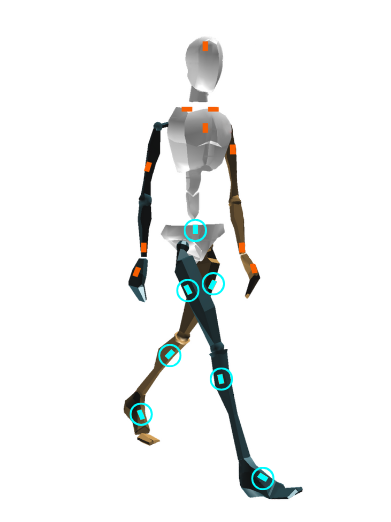
\includegraphics[width=0.33\linewidth]{figures/gab/lower limb config.png}
      \caption{Lower Limb Sensor Configuration}
      \label{fig:sub1}
    \end{subfigure}\hfill
    \begin{subfigure}{.5\textwidth}
      \centering
      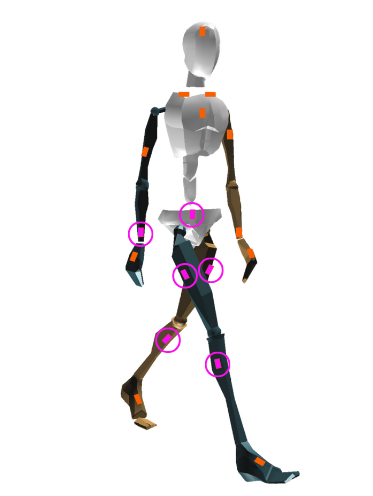
\includegraphics[width=0.33\linewidth]{figures/gab/luo config.png}
      \caption{Luo Sensor Configuration}
      \label{fig:sub2}
    \end{subfigure}
  \caption{Sensor Configurations}
    \label{fig:test}
    \end{figure}

\FloatBarrier

As for the IEE foot pressure insoles, there are 8 sensors available as part of the device. The locations on the insole are labeled as such: (Arch, Hallux, Heel L, Heel R, Met 1, Met 3, Met 5, Toes). For this study we included only the raw pressure data from the insoles. Another key area where the data was adjusted was in the downsizing of the classes that we considered. Originally there were 7 classes, but for our interests in clinical relevancy in this study we removed the two classes “pavement\_up” and “pavement\_down” so that we retained only 5 classes. Additionally, the IMU data was expressed in the global coordinate system. To ensure consistency and physiological interpretability, we rotated the data into each sensor's local coordinate system using the quaternion orientation data provided by each sensor. The transformation was implemented using custom Python code, which is available at \href{https://github.com/jillemmerzaal/heading-direction}{this repository}. For both approaches we sought out to test four different models: IMU sensors in Lower Limb configuration, IMU sensors in Luo configuration, foot pressure insoles, and IMU sensors in Lower Limb configuration combined with foot pressure insoles. 



% \begin{table}[ht]
%     \centering
%     \caption{Performance Metrics Formulas}
%     \begin{tabular}{l c}
%         \hline
%         \textbf{Metric} & \textbf{Formula} \\
%         \hline
%         Accuracy & \( \frac{TP + TN}{TP + TN + FP + FN} \) \\[2ex]
%         F1 Score & \( \frac{2 \cdot \text{Precision} \cdot \text{Recall}}{\text{Precision} + \text{Recall}} \) \\[2ex]
%         Sensitivity (Recall) & \( \frac{TP}{TP + FN} \) \\[2ex]
%         Specificity & \( \frac{TN}{TN + FP} \) \\[2ex]
%         \hline
%     \end{tabular}
% \end{table}

% \FloatBarrier


\subsubsection{Data Segmentation}
We implemented two distinct strategies for data segmentation and evaluated their performance separately. The first strategy involved gait event detection using annotations from the dataset derived from the insole sensors. These annotations identified instances when the foot pressure insoles were in contact with the ground. To validate these annotations, the insole pressure measurements were evaluated and compared when implementing a threshold to indicate step or not. These annotations facilitated the segmentation of gait cycles (n=29,988), allowing for the extraction of features from each cycle individually. Each of these gait cycles were then interpolated to a length of 100 rows. The second strategy employed a sliding window approach with a window size of 2 seconds and a step size of 1 second, resulting in the segmentation of 30444 windows.  The window and step sizes were chosen to maintain a nearly similar number of windows and gait cycles from the first strategy to ensure that any differences in performance could not be attributed to variations in input segment length.

\subsection{Machine Learning Approach}
\subsubsection{Feature Engineering and Reduction}
Feature engineering was performed prior to model development using the Python 3.10 (Python Software Foundation) packages Pandas \cite{reback2020pandas}, Numpy \cite{harris2020array} and Scikit-learn \cite{scikit-learn}.

% Prior to feature calculation, additional features related to orientation and elevation changes were introduced. The elevation difference between consecutive data points was approximated by processing the pelvis acceleration signal on the z-axis. This signal was integrated over time (60 Hz sampling frequency) to calculate velocity and then integrated again to estimate position. The difference in position between consecutive data points was used to determine elevation changes.

% For orientation, gyroscope data from the pelvis sensor along all three axes (x, y, z) were used. These data provided rotational velocities, which were integrated to compute orientation angles. To reduce noise, a second-order low-pass Butterworth filter with a cutoff frequency of 5 Hz was applied before integration. The use of IMUs mounted on the pelvis for tracking three-dimensional orientation angles has been validated in prior studies \cite{proceedings2020049010}.

Statistical features were calculated for each gait cycle, including minimum, maximum, mean, standard deviation, IQR, mean absolute deviation (MAD), area under the curve (AUC), skewness, kurtosis, and entropy using a histogram-based method with 10 bins. Frequency-based features were also included, such as the first five discrete Fourier transform (DFT) coefficients and the weighted mean frequency.
Feature reduction was performed using filter methods to optimize the dataset. Features with a correlation threshold of 0.8 or higher were discarded, retaining only the first feature of each correlated set. Features with no variation across the dataset and those with a low variation coefficient (less than 0.1) were also removed.

\subsubsection{Model Training and Evaluation}

The preprocessed and reduced dataset was split into training (80\%) and test (20\%) sets using a subject-wise splitting approach to ensure that all data from a single participant were exclusively in either the training or the test set \cite{Saeb2017}. The XGBoost algorithm \cite{chen2016xgboost} was selected as the machine learning model for surface classification due to its robustness and high performance in structured data classification tasks. To tune the hyperparameters, we implemented a Stratified Group k-Fold cross-validation approach. This method ensured that the train and validation folds did not contain data from the same participant, reducing the risk of data leakage and improving the model's generalizability. A grid search was conducted to optimize hyperparameters such as learning rate, maximum depth, and the number of estimators.

Model performance was evaluated using several metrics: accuracy, F1 score, sensitivity, and specificity. Sensitivity and specificity were included to align with clinical evaluation standards. 
% Confusion matrices were generated to assess classification performance across different surface types, providing insights into misclassification rates. The XGBoost model demonstrated high performance in distinguishing between various surfaces, with sensitivity and specificity indicating its applicability in clinical and real-world scenarios.


\subsection{Deep Learning approach}

To classify walking modes based on wearable sensor data, a deep learning pipeline was developed using a one-dimensional convolutional neural network (1D-CNN) since it is particularly well-suited for this task because it effectively captures local temporal patterns in sequential sensor data \cite{ref1dcnn}. We employed the same subject-wise data split as the machine learning approach to ensure uniformity. Feature columns were standardized using a StandardScaler, and categorical walking labels were encoded using a LabelEncoder and one-hot encoding. A CNN architecture was defined and tuned using Keras Tuner’s random search strategy, optimizing hyperparameters such as the number of filters, kernel size, dense layer units, dropout rate, and learning rate. The model was trained using a categorical cross-entropy loss function and Adam optimizer, with class weights applied to address label imbalance. Early stopping was employed to prevent overfitting. Model performance was evaluated on the held-out test set using the same evaluation metrics as the machine learning approach.
% The model architecture is shown in Figure~\ref{fig:cnn_architecture}.

% \begin{figure}[ht]
%     \centering
%     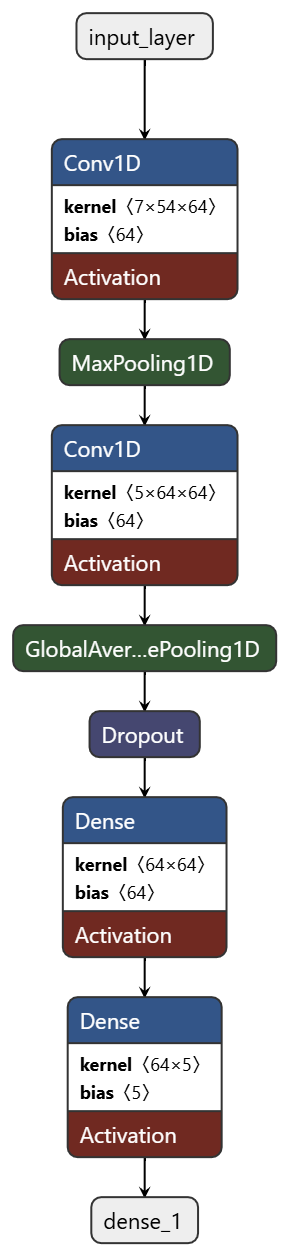
\includegraphics[width=0.25\linewidth]{figures/oussama/best_model_tf_format.h5.png}
%     \caption{Architecture of the 1D Convolutional Neural Network (1D-CNN) used for walking mode classification.}
%     \label{fig:cnn_architecture}
% \end{figure}

%%%%%%%%%%%%%%%%%%%%%%%%%%%%%%%%%%%%%%%%%%
\section{Results}
\label{sec:Results}


\begin{table}[ht]
\centering
\caption{Performance Metrics for Different Sensor Configurations of the Machine Learning Approach}
\resizebox{\textwidth}{!}{
\begin{tabular}{llcccc}
\hline
\textbf{Segmentation} & \textbf{Sensor Configuration} & \textbf{Accuracy} & \textbf{F1 Score} & \textbf{Sensitivity} & \textbf{Specificity} \\ 
\hline
\multirow{4}{*}{\textbf{Gait}} 
& \textbf{Xsens\_lower\_limbs}        & \textbf{0.92} & \textbf{0.92} & \textbf{0.90} & \textbf{0.96} \\ 
& Xsens\_luo                          & 0.91          & 0.92          & 0.89          & 0.96          \\  
& Pressure\_insoles                   & 0.76          & 0.71          & 0.67          & 0.91          \\  
& Pressure\_insoles + Xsens\_lower\_limbs & 0.90     & 0.91          & 0.88          & 0.96 \\
\hline
\multirow{4}{*}{\textbf{Sliding Window}} 
& \textbf{Xsens\_lower\_limbs}        & \textbf{0.87} & \textbf{0.88} & \textbf{0.86} & \textbf{0.95} \\
& Xsens\_luo                          & 0.86          & 0.88          & 0.85          & 0.95          \\ 
& Pressure\_insoles                   & 0.71          & 0.55          & 0.52          & 0.89          \\ 
& Pressure\_insoles + Xsens\_lower\_limbs & 0.87     & 0.87          & 0.84          & 0.95 \\
\hline
\end{tabular}%
}
\label{tab:ml_gait_cycle_seg}
\end{table}

\begin{table}[ht]
\centering
\caption{Performance Metrics for Different Sensor Configurations of the Deep Learning Approach}
\resizebox{\textwidth}{!}{
\begin{tabular}{llcccc}
\hline
\textbf{Segmentation} & \textbf{Sensor Configuration} & \textbf{Accuracy} & \textbf{F1 Score} & \textbf{Sensitivity} & \textbf{Specificity} \\ 
\hline
\multirow{4}{*}{\textbf{Gait}} 
& Xsens\_lower\_limbs                     & 0.88 & 0.86 & 0.83 & 0.95 \\
& Xsens\_luo                              & 0.84 & 0.82 & 0.77 & 0.93 \\
& Pressure\_insoles                       & 0.63 & 0.47 & 0.45 & 0.87 \\
& \textbf{Pressure\_insoles + Xsens\_lower\_limbs} & \textbf{0.91} & \textbf{0.91} & \textbf{0.88} & \textbf{0.96} \\
\hline
\multirow{4}{*}{\textbf{Sliding Window}} 
& \textbf{Xsens\_lower\_limbs}                     & \textbf{0.94} & \textbf{0.93} & \textbf{0.93} & \textbf{0.97} \\
& Xsens\_luo                              & 0.91 & 0.90 & 0.89 & 0.96 \\
& Pressure\_insoles                       & 0.61 & 0.44 & 0.41 & 0.85 \\
& Pressure\_insoles + Xsens\_lower\_limbs & 0.91 & 0.91 & 0.88 & 0.96 \\
\hline
\end{tabular}%
}
\label{tab:dl_gait_cycle_seg}
\end{table}
Tables \ref{tab:ml_gait_cycle_seg} and \ref{tab:dl_gait_cycle_seg} summarize the performance of machine learning (ML) and deep learning (DL) models for gait segmentation using different sensor configurations and segmentation strategies. Overall, models using Xsens lower limbs achieved the highest accuracy and F1 scores across both ML and DL methods. Combining pressure insoles with Xsens generally improved performance compared to pressure insoles alone. DL with a sliding window approach yielded the best performance overall (accuracy = 0.94, F1 = 0.93), particularly with Xsens lower limb data. In contrast, pressure insoles alone consistently resulted in lower performance, with F1 scores as low as 0.44–0.55 depending on the method.

\FloatBarrier
%%%%%%%%%%%%%%%%%%%%%%%%%%%%%%%%%%%%%%%%%%
\section{Discussion}
This study investigates the performance of different sensor configurations and segmentation strategies in classifying walking conditions using machine learning and deep learning models. Our findings strongly support the first hypothesis, confirming that IMU sensors provide more discriminative information than pressure insoles across both modeling approaches. The second hypothesis, that combining IMU and pressure insole data would enhance model performance, was partially supported. While sensor fusion consistently outperformed pressure insoles alone and occasionally improved over IMU-only configurations, the gains were modest, suggesting limited additive value from pressure data. The third hypothesis, that gait cycle segmentation would improve model performance, was conditionally supported. Gait segmentation yielded higher accuracy for machine learning models, likely due to the structured features extracted per gait cycle, whereas deep learning models benefitted more from the sliding window approach. These results highlight the importance of selecting the appropriate segmentation method based on the model type and suggest that while pressure insoles contribute complementary data, IMU sensors remain the primary source of informative gait features.

Across sensor configurations, models using IMU data consistently outperformed those using pressure insoles alone, confirming the discriminative strength of inertial measurements in classifying walking conditions. The highest F1-scores for IMU-based models reached 0.92 with machine learning and 0.93 with deep learning. In contrast, pressure insoles alone yielded substantially lower performance, with peak F1-scores of 0.71 for machine learning and 0.47 for deep learning. Combining IMU and insole data resulted in performance that was comparable to IMU-only models, though it did not consistently improve results. This suggests that while pressure insoles provide complementary gait information, their integration with IMU data may not significantly enhance classification unless additional biomechanical features or more advanced fusion strategies are incorporated.

The segmentation strategy also significantly influenced model performance: machine learning models benefited more from gait-cycle-based segmentation, likely due to the meaningful handcrafted features extracted over entire gait cycles, whereas deep learning models achieved superior results with sliding windows, which preserve temporal continuity suitable for convolutional operations. Moreover, the Luo sensor configuration (which replaces the feet sensors in the lower limb setup with a right forearm sensor while retaining the pelvis, upper legs, and lower legs) achieved performance comparable to the full lower limb configuration. This finding highlights its potential as a practical alternative in settings where foot-mounted sensors may be inconvenient or less feasible. The similar performance suggests that upper-limb motion (captured via the forearm) may offer useful complementary information to lower-body kinematics. In contrast, models relying solely on pressure insoles consistently underperformed, particularly in deep learning scenarios, underscoring their limited capacity to capture the full-body dynamics required for accurate surface classification.

Alternative segmentation techniques, such as adaptive windowing based on step detection or surface agnostic step-detection from IMU sensor data are an area of future exploration if you are interested in applying the machine learning techniques. While our gait cycles were segmented by insole pressure data, perhaps segmenting based on IMU gathered data provides an additional insight, and thereby limiting the equipment requirements. Also alternatives to feature selection from fused sensors should be explored. 
As for the deep learning methods, certain tools can be applied to allow for better explainability and add transparency to the black-box models. This is particularly important as clinicians and patients alike want to further understand better the why and how these pathologies are affecting the patients rather than just the binary information that they are being affected.

In comparison with previous work, our results show an improvement in the classification of outdoor irregular walking surfaces. 
Our models show an improvement to previous works by Chen et al. \cite{Chen2019}, Hu et al. \cite{Hu_2021}, and Shah et al. \cite{Shah_2022}, allowing for an overall better performing model using less covariates, at more clinically relevant surfaces, recorded in a context that imitates real life walking conditions. Shah et al. \cite{Shah_2022} found an excellent F1-score of 0.96 using a CNN model with only the right shank sensor; however, in order to achieve that model performance, they needed participant calibration data during model training. Removing all calibration data from the training set, reduced the F1-score to XXXXX. Within a clinical setting, it is not always feasible to obtain surface calibration per participant. Within our data processing we used subject-wise stratification, thereby ensuring that no calibration data of the participants were in the training set and maintaining comparable F1-scores. Future work, should investigate methods to enhance performance from single or dual sensor models, without relying on calibrating the data. Furthermore, more effort needs to be placed on the calculation and extraction of relevant features using insole pressure data as this would allow for efficiency in data collection as well as patient compliance.

\subsection{Limitations}

There are several limitations that warrant discussion. First in the machine learning model, we relied on generic (statistical) features instead of domain specific-features. This may have hindered the model's ability to fully leverage the available gait information. This was done intentionally to allow for direct method comparison with the performance of the deep learning model, and we sought to explore how much we could understand given the raw signals. Perhaps incorporating (biomechanical) domain-specific features from the insole data would provide the models with more concise information to improve its predictive performances. 
We also mainly relied on statistical features and did not incorporate advanced feature selection techniques such as the Salp Swarm Algorithm (SSA), as used in Chauhan et al. \cite{chauhan2025classifying}, which effectively reduced feature dimensionality while maintaining high accuracy. Furthermore, convolutional feature extraction was not explored in our study, which has been shown to improve performance in similar classification tasks. Future work could investigate the impact of deep learning-based feature extraction or optimization algorithms such as SSA to further refine our model performance.
Expanding studies to different populations remains a very important area for exploration. This study has only been done on healthy adults, limiting the generalizability to other populations. This work need to be continued on participants with musculoskeletal or neurological injury for these models to be applicable in clinical biomechanics in free living environments.
In addition, the selection and customization of specific surface conditions depending on the pathologies or injuries (soft surfaces, slippery surfaces, uneven surfaces) and reduced sensor placements will also help validate these findings and improve real-world applicability.

Second, we only focused on two model architectures: a 1D Convolutional Neural Network (1D CNN) for the deep learning approach and XGBoost for the machine learning approach. The 1D CNN was chosen for its effectiveness in capturing local temporal patterns in sequential sensor data while maintaining a relatively low computational cost compared to more complex architectures like Bi-CNN LSTM. Its structure is well-suited for processing multivariate time series such as IMU and pressure insole data, making it an efficient and interpretable choice for our classification task. XGBoost was selected for its strong performance with structured feature-based data, robustness to overfitting, and efficiency in handling high-dimensional input. Although we limited our exploration to these two well-established architectures to maintain a focused and interpretable evaluation, future work may benefit from exploring alternative or more advanced models tailored to specific sensor modalities.

\subsection{Code Availability}

The custom python notebooks for pre-processing the data as well as the model creations are provided in this \href{https://github.com/mcgillmotionlab/SurfaceClassification_FootPressure_IMU/tree/oussama/code}{Github repository}.

%%%%%%%%%%%%%%%%%%%%%%%%%%%%%%%%%%%%%%%%%%
\authorcontributions{For research articles with several authors, a short paragraph specifying their individual contributions must be provided. The following statements should be used ``Conceptualization, X.X. and Y.Y.; methodology, X.X.; software, X.X.; validation, X.X., Y.Y. and Z.Z.; formal analysis, X.X.; investigation, X.X.; resources, X.X.; data curation, X.X.; writing---original draft preparation, X.X.; writing---review and editing, X.X.; visualization, X.X.; supervision, X.X.; project administration, X.X.; funding acquisition, Y.Y. All authors have read and agreed to the published version of the manuscript.'', please turn to the  \href{http://img.mdpi.org/data/contributor-role-instruction.pdf}{CRediT taxonomy} for the term explanation. Authorship must be limited to those who have contributed substantially to the work~reported.}

\funding{Please add: ``This research received no external funding'' or ``This research was funded by NAME OF FUNDER grant number XXX.'' and  and ``The APC was funded by XXX''. Check carefully that the details given are accurate and use the standard spelling of funding agency names at \url{https://search.crossref.org/funding}, any errors may affect your future funding.}

\institutionalreview{In this section, you should add the Institutional Review Board Statement and approval number, if relevant to your study. You might choose to exclude this statement if the study did not require ethical approval. Please note that the Editorial Office might ask you for further information. Please add “The study was conducted in accordance with the Declaration of Helsinki, and approved by the Institutional Review Board (or Ethics Committee) of NAME OF INSTITUTE (protocol code XXX and date of approval).” for studies involving humans. OR “The animal study protocol was approved by the Institutional Review Board (or Ethics Committee) of NAME OF INSTITUTE (protocol code XXX and date of approval).” for studies involving animals. OR “Ethical review and approval were waived for this study due to REASON (please provide a detailed justification).” OR “Not applicable” for studies not involving humans or animals.}

\informedconsent{Any research article describing a study involving humans should contain this statement. Please add ``Informed consent was obtained from all subjects involved in the study.'' OR ``Patient consent was waived due to REASON (please provide a detailed justification).'' OR ``Not applicable'' for studies not involving humans. You might also choose to exclude this statement if the study did not involve humans.

Written informed consent for publication must be obtained from participating patients who can be identified (including by the patients themselves). Please state ``Written informed consent has been obtained from the patient(s) to publish this paper'' if applicable.}

\dataavailability{We encourage all authors of articles published in MDPI journals to share their research data. In this section, please provide details regarding where data supporting reported results can be found, including links to publicly archived datasets analyzed or generated during the study. Where no new data were created, or where data is unavailable due to privacy or ethical restrictions, a statement is still required. Suggested Data Availability Statements are available in section ``MDPI Research Data Policies'' at \url{https://www.mdpi.com/ethics}.} 

% Only for journal Drones
%\durcstatement{Current research is limited to the [please insert a specific academic field, e.g., XXX], which is beneficial [share benefits and/or primary use] and does not pose a threat to public health or national security. Authors acknowledge the dual-use potential of the research involving xxx and confirm that all necessary precautions have been taken to prevent potential misuse. As an ethical responsibility, authors strictly adhere to relevant national and international laws about DURC. Authors advocate for responsible deployment, ethical considerations, regulatory compliance, and transparent reporting to mitigate misuse risks and foster beneficial outcomes.}

% Only for journal Nursing Reports
%\publicinvolvement{Please describe how the public (patients, consumers, carers) were involved in the research. Consider reporting against the GRIPP2 (Guidance for Reporting Involvement of Patients and the Public) checklist. If the public were not involved in any aspect of the research add: ``No public involvement in any aspect of this research''.}
%
%% Only for journal Nursing Reports
%\guidelinesstandards{Please add a statement indicating which reporting guideline was used when drafting the report. For example, ``This manuscript was drafted against the XXX (the full name of reporting guidelines and citation) for XXX (type of research) research''. A complete list of reporting guidelines can be accessed via the equator network: \url{https://www.equator-network.org/}.}
%
%% Only for journal Nursing Reports
%\useofartificialintelligence{Please describe in detail any and all uses of artificial intelligence (AI) or AI-assisted tools used in the preparation of the manuscript. This may include, but is not limited to, language translation, language editing and grammar, or generating text. Alternatively, please state that “AI or AI-assisted tools were not used in drafting any aspect of this manuscript”.}

\acknowledgments{In this section you can acknowledge any support given which is not covered by the author contribution or funding sections. This may include administrative and technical support, or donations in kind (e.g., materials used for experiments). Where GenAI has been used for purposes such as generating text, data, or graphics, or for study design, data collection, analysis, or interpretation of data, please add “During the preparation of this manuscript/study, the author(s) used [tool name, version information] for the purposes of [description of use]. The authors have reviewed and edited the output and take full responsibility for the content of this publication.”}

\conflictsofinterest{Declare conflicts of interest or state ``The authors declare no conflicts of interest.'' Authors must identify and declare any personal circumstances or interest that may be perceived as inappropriately influencing the representation or interpretation of reported research results. Any role of the funders in the design of the study; in the collection, analyses or interpretation of data; in the writing of the manuscript; or in the decision to publish the results must be declared in this section. If there is no role, please state ``The funders had no role in the design of the study; in the collection, analyses, or interpretation of data; in the writing of the manuscript; or in the decision to publish the results''.} 

%%%%%%%%%%%%%%%%%%%%%%%%%%%%%%%%%%%%%%%%%%
%% Optional

%% Only for journal Encyclopedia
%\entrylink{The Link to this entry published on the encyclopedia platform.}

\abbreviations{Abbreviations}{
The following abbreviations are used in this manuscript:
\\

\noindent 
\begin{tabular}{@{}ll}
MDPI & Multidisciplinary Digital Publishing Institute\\
DOAJ & Directory of open access journals\\
TLA & Three letter acronym\\
LD & Linear dichroism
\end{tabular}
}

%%%%%%%%%%%%%%%%%%%%%%%%%%%%%%%%%%%%%%%%%%
%% Optional
\appendixtitles{no} % Leave argument "no" if all appendix headings stay EMPTY (then no dot is printed after "Appendix A"). If the appendix sections contain a heading then change the argument to "yes".
\appendixstart
\appendix
\section[\appendixname~\thesection]{}
\subsection[\appendixname~\thesubsection]{}
The appendix is an optional section that can contain details and data supplemental to the main text---for example, explanations of experimental details that would disrupt the flow of the main text but nonetheless remain crucial to understanding and reproducing the research shown; figures of replicates for experiments of which representative data are shown in the main text can be added here if brief, or as Supplementary Data. Mathematical proofs of results not central to the paper can be added as an appendix.

\begin{table}[H] 
\caption{This is a table caption.\label{tab5}}
%\newcolumntype{C}{>{\centering\arraybackslash}X}
\begin{tabularx}{\textwidth}{CCC}
\toprule
\textbf{Title 1}	& \textbf{Title 2}	& \textbf{Title 3}\\
\midrule
Entry 1		& Data			& Data\\
Entry 2		& Data			& Data\\
\bottomrule
\end{tabularx}
\end{table}

\section[\appendixname~\thesection]{}
All appendix sections must be cited in the main text. In the appendices, Figures, Tables, etc. should be labeled, starting with ``A''---e.g., Figure A1, Figure A2, etc.

%%%%%%%%%%%%%%%%%%%%%%%%%%%%%%%%%%%%%%%%%%
%\isPreprints{}{% This command is only used for ``preprints''.
\begin{adjustwidth}{-\extralength}{0cm}
%} % If the paper is ``preprints'', please uncomment this parenthesis.
%\printendnotes[custom] % Un-comment to print a list of endnotes

\reftitle{References}

% Please provide either the correct journal abbreviation (e.g. according to the “List of Title Word Abbreviations” http://www.issn.org/services/online-services/access-to-the-ltwa/) or the full name of the journal.
% Citations and References in Supplementary files are permitted provided that they also appear in the reference list here. 

%=====================================
% References, variant A: external bibliography
%=====================================
% \bibliography{your_external_BibTeX_file}

%=====================================
% References, variant B: internal bibliography
%=====================================

\bibliographystyle{elsarticle-num} 
\bibliography{cas-refs}
% ACS format

%%%%%%%%%%%%%%%%%%%%%%%%%%%%%%%%%%%%%%%%%%
\PublishersNote{}
%\isPreprints{}{% This command is only used for ``preprints''.
\end{adjustwidth}
%} % If the paper is ``preprints'', please uncomment this parenthesis.
\end{document}

